\subsection{A customer successfully purchases gas and charges it on
a monthly bill}

The sequence diagram is shown on figure~\ref{fig:seq-diagram1}

\begin{landscape}
    \begin{figure}[!ht]
        \centering
        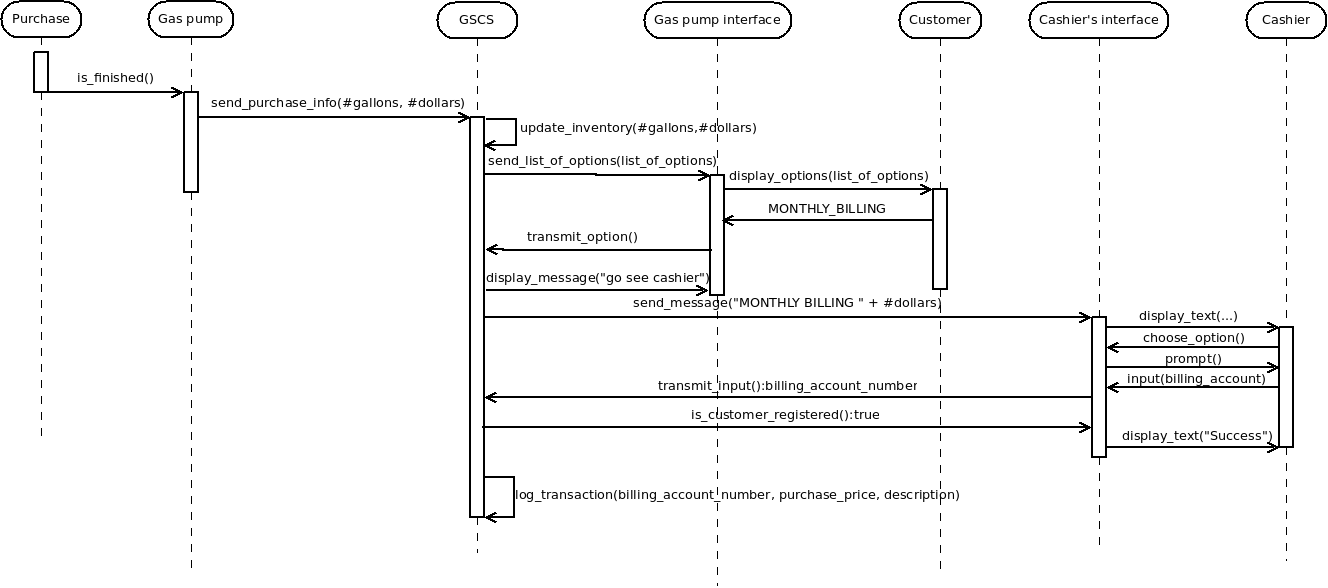
\includegraphics[width=\linewidth]{drafts/sequence_1.png}
        \caption{A customer succesfully purchases gas and charges it on a
        monthly bill}
        \label{fig:seq-diagram1}
    \end{figure}
\end{landscape}

\subsection{A customer purchases gas and attempts to pay by credit
card but his card is refused. He then pays by cash to the cashier.}

The sequence diagram is shown on figure~\ref{fig:seq-diagram2}

\begin{landscape}
    \begin{figure}[!ht]
        \centering
        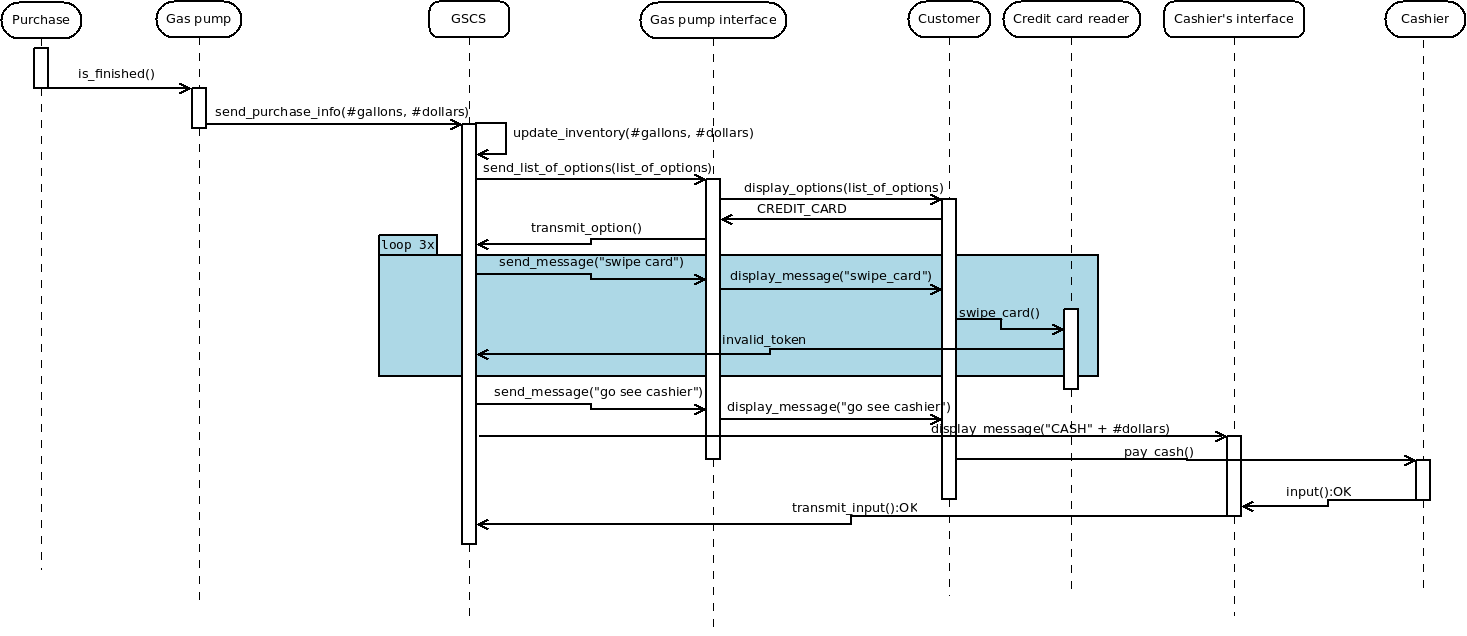
\includegraphics[width=\linewidth]{drafts/sequence_2.png}
        \caption{A customer purchases gas and attempts to pay by credit card but
        his card is refused. He then pays by cash to the cashier.}
        \label{fig:seq-diagram2}
    \end{figure}
\end{landscape}

\subsection{The cashier successfully processes a monthly payment by
credit card.}

The sequence diagram is shown on figure~\ref{fig:seq-diagram3}

\begin{landscape}
    \begin{figure}[!ht]
        \centering
        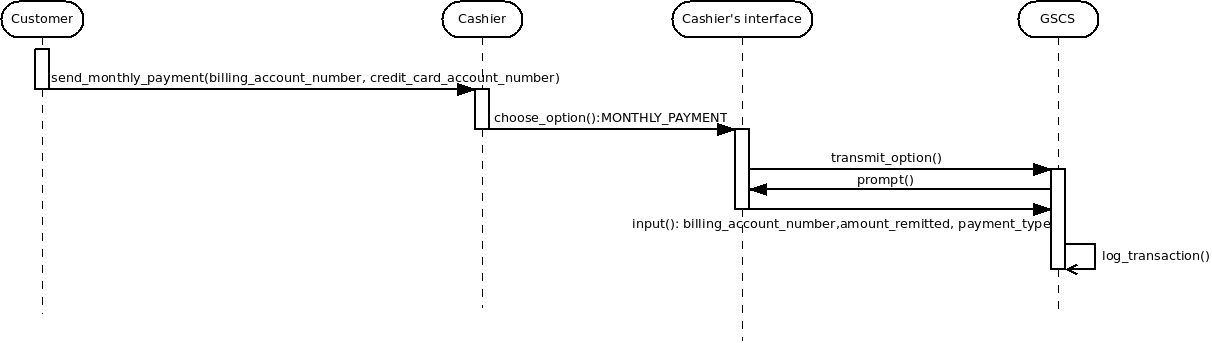
\includegraphics[width=\linewidth]{drafts/sequence_3.png}
        \caption{The cashier successfully processes a monthly payment by credit
        card.}
        \label{fig:seq-diagram3}
    \end{figure}
\end{landscape}
